\chapter{Design}
After analyzing the problem, this chapter will go through the design of the application architecture of our UIProtocol client. The design phase is of crucial importance as it is the time when important design decisions are made. In this phase, the application's architecture needs to be thought through so that its future extensions are relatively easy to implement and cost of maintenance is low.

From the analysis, we conclude requirements for the application which will be developed. Further on, the section describes the design of several sub-systems which are responsible for handling the communication, models, events, inner representation of the UI elements, their rendering and more. The chapter contains several UML diagrams. Note that most of them are simplified.

Even though there are existing implementations of UIProtocol client, the design of this one was not influenced by any of them.

\subsection{Requirements}
The client application will be developed and run on a Windows Phone 8 device. Since the entire user interfaces and information about events is intended to be transferred over wireless internet connection, there will be a delay present in the application's reaction time, which is a inescapable consequence of the client-server architecture. The delay should be reasonably small to allow for a comfortable usage of the application. Even with this delay, the application should perform well in terms of UI rendering times, reaction time and overall feel.

There is a number of requirements an app should meet in order to be truly accessible. In our analysis, we found that the support of Windows Phone 8 for accessibility is lower than at the competing platforms. Namely, support for a key accessibility feature, the screen reader, is not present by default. This can be a major flaw to the application accessibility – especially for visually impaired who would have to use a third-party screen reader in order to be able to navigate through the app\footnote{Windows Phone 8.1 users may use the Narrator feature}.

We may propose some new features that could be implemented by UIProtocol to increase its own support for accessibility. At any rate, even with the Windows Phone 8 platform's low accessibility support, the developed app will remain a functional UIP client capable of handling valid UIP documents.


\subsubsection{Summary of Requirements}
We have developed the following lists of non-functional and functional requirements, respectively.
\\\\
Non-functional requirements:
\begin{itemize}
  \item UI components have platform-native look
  \item Client app will be will be written in C\#
  \item The client should not use much phone resources when idle
  \item App should be stable and able to process valid UIP documents
  \item Compatibility with UIP specification, draft 8
  \item Ability to run on any WP8 device
  \item UI loading times below 0.5 s for UIs of usual size, with stable internet connections
\end{itemize}
~\\
Functional requirements:
\begin{itemize}
  \item  Support for basic user interface elements
  \item Graceful degradation for unsupported elements
  \item  Support for binding and model-wide binding
  \item  Support for interpolated model updates (animations)
  \item  Support for UI generator API
  \item  Support for Events
  \item Support for absolute and grid layouts
  \item Support for styling (font size, colors, etc.)
\end{itemize}

\subsection{Client-server Communication}
The client will communicate with the server over TCP connection which will be handled by a standard socket. Upon this communication channel, UIProtocol XML files will be transferred.

Once the client connects to the server and goes through the connection procedure described in \cite{uip}, the server sends the XMLs describing the UI. The UML diagram of the classes responsible for the communication is shown in figure \ref{fig:classComm}. Since some of the methods will only work with the passed parameters and not modify the object's state, they will be made static. 

\begin{figure}[ht!]
\centering
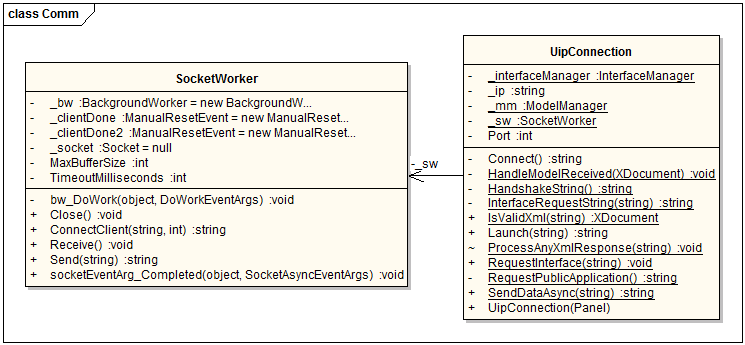
\includegraphics[width=145mm]{pics/3/classComm.png}
\caption{Class diagram of communication classes}
\label{fig:classComm}
\end{figure}

Apart from the mentioned classes that will serve for communicating the XML messages, there there will be another class responsible for acquiring resources (such as images) from the server. For this purpose, the server is awaiting a HTTP connection on another port and the client can open a connection and make a standard HTTP request for the resource. This functionality will be implemented in the \texttt{HttpConnection} class.

\subsection{Parsing XML Into Inner Object Representation}
After the UIP documents will be received by the \texttt{UipConnection} class, they will be passed to instances of \texttt{ModelManager} and \texttt{InterfaceManager} classes.\linebreak \texttt{ModelManager} will be responsible for processing possible new models or model updates and will be discussed later in more detail.

All of the UIP elements need to be represented by objects, so that they are easily manipulated. To create the object representation, \texttt{InterfaceManager} class will process the XML data that describes the UI by recursively traversing the XML tree and creating instances of \texttt{Interface}, \texttt{Container} and \texttt{Element} classes, based on the type of the considered XML node. These instances will represent the UIP elements of the same name - UIP interface, UIP container and UIP element, respectively. This way, every UIP element will be parsed into an inner object representation that will be easy to handle in further work with the objects.

\begin{figure}[ht!]
\centering
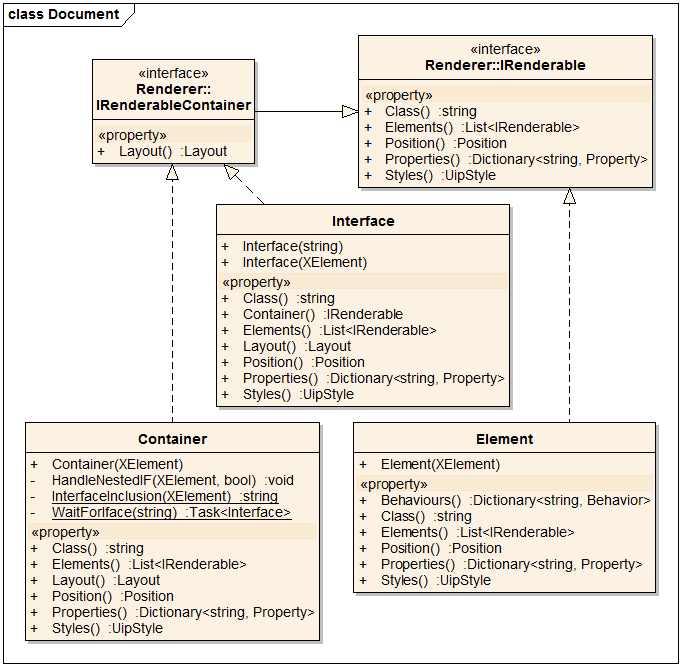
\includegraphics[width=145mm]{pics/3/classDocument2.png}
\caption{Class diagram of the classes representing UIP interface, container and element}
\label{fig:classDocument}
\end{figure}

An important component is the \texttt{IRenderable} interface which is implemented by the \texttt{Interface}, \texttt{Container} and \texttt{Element} classes. This interface represents the functionality all of the classes have in common - most importantly the UIP class (i.e. type of the UI control - see \ref{uipProperty} for example of \texttt{public.input.text} which represents the C\#'s \texttt{TextBox}), UIP properties and contained elements. \texttt{IRenderableContainer} only extends the \texttt{IRenderable} interface by adding a method for obtaining layout. Since layout is a container feature, only \texttt{Interface} and \texttt{Container} classes will implement it.

\subsection{Managing Models and Binding}
To conform the UIP specification, the client must be thin, i.e. it will only store as much data as is needed to render the required interfaces and not execute any code on that data. The data shown to the user can be either constant or come from models, which are designed to be a data storage, as discussed in \ref{subsec:models}. Models will be managed by one instance of \texttt{ModelManager} class.

If an UIP element has a property that refers to a model, \texttt{ModelManager} will be responsible for requesting the model containing this property. Once the model is received, \texttt{ModelManager} will store all its properties and will manage future model updates. Note that the updates can come from the server at any time. \texttt{ModelManager} will also need a reference to \texttt{InterfaceManager} because server's models can contain a request to render an interface. The relationship between classes that are involved in model management is shown in figure \ref{fig:classModel}.

When a UIP property refers to a model, a binding will be created so that when the UIP property is updated, the update is shown in the UI. For that reason there has to be a data binding between the two. We will make use of the data binding API which is built-in to the Windows Phone platform.

\begin{figure}[ht!]
\centering
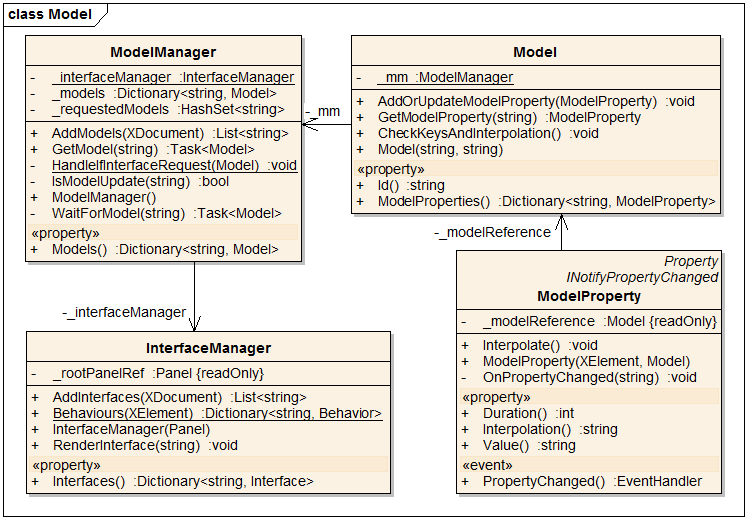
\includegraphics[width=145mm]{pics/3/classModel.png}
\caption{Model and interface management class diagram}
\label{fig:classModel}
\end{figure}

\subsection{Managing Interfaces}
Interface is the root element for all UI controls in UIP documents. An application can contain a large number of interfaces. We therefore need a class to keep the interface information. \texttt{InterfaceManager} will serve as a place for storing information about received and requested interfaces. The most important methods implemented in it will be for adding received interfaces, obtaining an interface and rendering. The process of rendering is described more closely in the next paragraph.

\subsection{Rendering the UI}
The information about UI elements comes from the server in form of XML description. This description is parsed into inner object representation - classes shown in figure \ref{fig:classDocument}. 

After this is done, \texttt{InterfaceManager} will call the \texttt{Render()} method of the \texttt{Renderer} class. This method will traverse the tree of the newly created instances of classes from figure \ref{fig:classDocument} and for each one creates a new class instance which will wrap the platform-native UI controls, as described in the next section.

\begin{figure}[ht!]
\centering
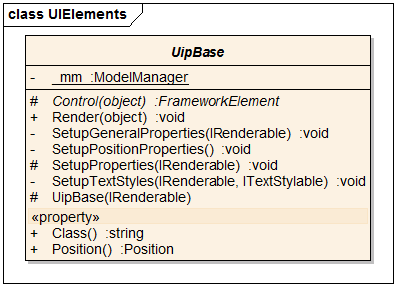
\includegraphics[width=85mm]{pics/3/classUipBase.png}
\caption{UipBase class diagram}
\label{fig:classUipBase}
\end{figure}

\subsection{Representing the Platform-native UI Components}
There is one more step toward the controls that are rendered to the user which involves the transition from the inner object representation to the platform-native components.

The platform-native components will be wrapped into wrapper classes whose names will indicate the component which is wrapped inside (i.e. \texttt{UipPasswordBox} will be the wrapper class of WP8's \texttt{PasswordBox}). There will be an abstract base class, \texttt{UipBase} which will contain everything the wrapper classes have in common: methods for binding to models, and support for styling, element dimensions and positioning.\\
Any particular UI element needs to inherit from the base class in order to support rendering, model updates and other functionality provided by the base class.

\subsection{Events}
The application is designed to support the client-to-server communication in form of events. Events are the only data sent by the client and their intent is to inform server of an user action or request missing data - models.\\\\
Events could be divided into two categories.\\
\begin{description}
  \item[Static] \hfill \\
 Events that are static and are hard-coded within the application. These events are used rarely, typically while going through the procedure of connecting to the server. Currently these are the \texttt{public.connection.connect} and \texttt{public.request. model}, as well as \texttt{public.application}.
  \item[Dynamic] \hfill \\
 Other events are the ones triggered by the user or by the client itself, when it requests a model. These events are dynamic, created at runtime. The event firing - i.e. notifying server of an action taking place, is a relatively simple process which will be handled by two classes. Its working is described in the Implementation chapter.
\end{description}

\begin{figure}[ht!]
\centering
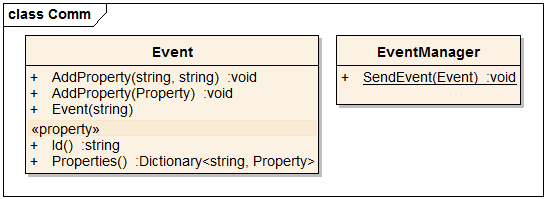
\includegraphics[width=120mm]{pics/3/classEvent.png}
\caption{event class diagram}
\label{fig:classEvent}
\end{figure}

\subsection{Properties}
Properties are the most nested objects in UIP documents. They are used extensively within many classes, including \texttt{Layout}, \texttt{Event} or \texttt{Element}. In all classes they will be stored in dictionaries, identified by their name. The \texttt{ModelProperty} class used in Model will inherit from \texttt{Property} class. 

%They are directly attached to the particular class instance.

\subsection{Layouts}
Windows Phone 8 supports two main types of layouts: absolute and dynamic.
In an absolute layout, child elements are arranged in a layout panel by specifying their exact locations relative to their parent element. Absolute positioning doesn't consider the size of the screen.

In a dynamic layout, the child elements are arranged by specifying how they should be arranged and how they should wrap relative to their parent. With dynamic layout, the user interface appears correctly on various screen resolutions.\\

Both layout types will be supported in our client. Even though absolute layout is not recommended by the accessibility guidelines \cite{wp8guide} it is a basic form of layout and decision has been made to support it.

Layouts are a feature of containers and interfaces which support it through the \texttt{IRenderableContainer} interface. Every container, therefore can place its content into one of the two layouts. As with any property, the positioning will be binding-enabled.

The client will support a container with scrollable content (through \texttt{ScrollViewer}) so that content which does not fit in the screen can be reached by scrolling.

\subsection{Configuration}
Client will have support for basic configuration - i.e. the default IP address and ports on which the socket is tying to connect to the UIP and the HTTP server. Also the constants which are used in the portions of XML throughout the application will be stored in one static class so that they are easy to maintain. 

\subsection{Behaviors}
Behaviors are used to attach event listeners to UI controls. C\# has a built-in support for events through Event and Delegate classes and we will take advantage of it.

Behaviors will be attached to the classes inheriting from \texttt{UipBase} as event handlers. Each handler is for one type of behavior and when the event is fired, the event handler catches it.

\subsection{Interpolation}
The client will support interpolation of UI controls. In the context of UIProtocol, interpolation means animation of UI elements. For example, some action may trigger interpolation which will cause an UI element to move on the screen of the phone. A model update will specify the direction, duration and position where the UI element should move. UIProtocol specifies multiple types of interpolation, our client will only support linear (\texttt{public.number.linear}) and immediate (\texttt{public.immediate}) interpolations.

%\begin{figure}[ht!]
%\centering
%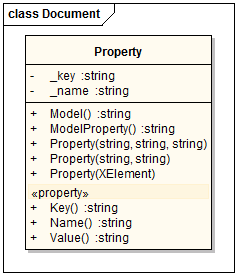
\includegraphics[width=60mm]{pics/3/classProperty.png}
%\caption{properties class diagram}
%\label{fig:classProperty}
%\end{figure}

%positions, interpolace
